% COMPOSITE

\subsection{Problem Set}

\subsubsection{(Problem 1) $\pm$ Resolving Vector Components with Trigonometry}

\problempart

Find the components of the vector $\vec{A}$ with length $a=1.00$ and angle $\alpha=\SI{15.0}{\degree}$ with respect to the $x$-axis as shown in the figure below.

\begin{center}
	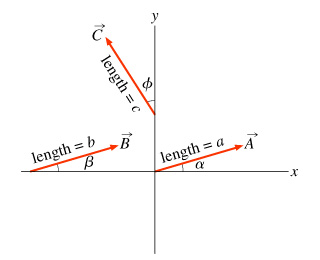
\includegraphics[width=0.5\textwidth]{/Users/max/course-manager/data/semester/Spring 2025/course/PHY2111/chapter/Vectors and Coordinate Systems/section/3.1-3.4/figures/figure_1.jpeg}
\end{center}

\begin{solution}
	\begin{align*}
		A_{x} &= 1.00 \cos 15.0 = 0.965925826289 \\
		A_{y} &= 1.00 \sin 15.0 = 0.258819045103
		.\end{align*}
\end{solution}

\problempart

Find the components of the vector $\vec{B}$ with length $b=1.00$ and angle $\beta = \SI{10.0}{\degree}$ with respect to the $x$ axis as shown in the figure.

\begin{solution}
	\begin{align*}
		B_{x} &= 1.00 \cos 10.0 = 0.984807753012 \\
		B_{y} &= 1.00 \sin 10.0 = 0.173648177667
		.\end{align*}
\end{solution}

\problempart

Find the components of the vector $\vec{C}$ with length $c=1.00$ and angle $\phi = \SI{35.0}{\degree}$ as shown in the figure.

\begin{solution}
	The angle with respect to the $x$ axis would be
	\[
		90 + 35 = 125
		.\]
	\begin{align*}
		C_{x} &= 1.00 \cos 125 = -0.573576436351 \\
		C_{y} &= 1.00 \sin 125 = 0.819152044289
		.\end{align*}
\end{solution}

\newpage

\subsubsection{(Problem 2) Problem 3.3 -- Enhanced -- with Hints and Feedback}

\begin{center}
	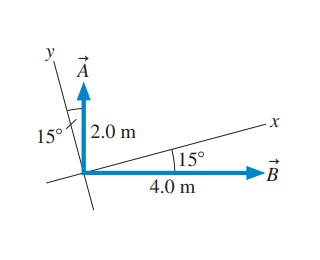
\includegraphics[width=0.5\textwidth]{/Users/max/course-manager/data/semester/Spring 2025/course/PHY2111/chapter/Vectors and Coordinate Systems/section/3.1-3.4/figures/figure_2.jpg}
\end{center}

\setcounter{partcounter}{2}
\paragraph{Parts A-B}

What are the $x$ and $y$ components of the vector $\vec{E}$ in terms of the angle $\theta$ and the magnitude $E$ shown in the figure above? Express your answers in terms of some or all of the variables $\theta$, $E$.

\begin{solution}
	\begin{align*}
		E_{x} &= E \cos \left( \frac{3\pi}{2} + \theta \right) \\
		E_{y} &= E \sin \left( \frac{3\pi}{2} + \theta \right)
		.\end{align*}
\end{solution}

\setcounter{partcounter}{4}
\paragraph{Parts C-D}

For the same vector, what are the $x$ and $y$ components in terms of the angle $\phi$ and the magnitude $E$?
Express your answers in terms of some or all of the variables $\phi$, $E$.

\begin{solution}
	\begin{align*}
		E_{x} &= E \cos \left( 2\pi - \phi \right) \\
		E_{y} &= E \sin \left( 2\pi - \phi \right)
		.\end{align*}
\end{solution}

\newpage

\subsubsection{(Problem 3) Problem 3.7 -- Enhanced -- with Hints and Feedback}

\setcounter{partcounter}{2}
\paragraph{Parts A-B}

Find the $x$ and $y$ components of $\vec{v} = \SI{9.5}{\frac{m}{s}}$, $\SI{30}{\degree}$ clockwise from the positive $y$ axis.

\begin{solution}
	\begin{align*}
		v_{x} &= \SI{9.5}{\frac{m}{s}} \cos \left( \SI{90}{\degree} - \SI{30}{\degree} \right) = \SI{4.75}{\frac{m}{s}}\\
		v_{y} &= \SI{9.5}{\frac{m}{s}} \sin \left( \SI{90}{\degree} - \SI{30}{\degree} \right) = \SI{8.23}{\frac{m}{s}}
		.\end{align*}
\end{solution}

\setcounter{partcounter}{4}
\paragraph{Parts C-D}

Find the $x$ and $y$ components of $\vec{a} = \SI{1.7}{\frac{m}{s^2}}$, \SI{30}{\degree} above the negative $x$-axis.

\begin{solution}
	\begin{align*}
		a_{x} &= \SI{1.7}{\frac{m}{s^2}} \cos \left( \SI{180}{\degree} - \SI{30}{\degree} \right) = \SI{-1.47}{\frac{m}{s^2}} \\
		a_{y} &= \SI{1.7}{\frac{m}{s^2}} \sin \left( \SI{180}{\degree} - \SI{30}{\degree} \right) = \SI{0.85}{\frac{m}{s^2}}
		.\end{align*}
\end{solution}

\setcounter{partcounter}{6}
\paragraph{Parts E-F}

Find the $x$ and $y$ components of $\vec{F} = \SI{60.0}{N}$, \SI{36.9}{\degree} counterclockwise from the positive $y$-axis.

\begin{solution}
	\begin{align*}
		F_{x} &= \SI{60.0}{N} \cos \left( \SI{90}{\degree} + \SI{36.9}{\degree} \right) = \SI{-36.03}{N} \\
		F_{y} &= \SI{60.0}{N} \sin \left( \SI{90}{\degree} + \SI{36.9}{\degree} \right) = \SI{47.98}{N}
		.\end{align*}
\end{solution}

\newpage

\subsubsection{(Problem 4) $\pm$ Vector Addition and Subtraction}

Let vectors
\begin{align*}
	\vec{A} &= \left( 1,0,-3 \right) \\
	\vec{B} &= \left( -2,5,1 \right) \\
	\vec{C} &= \left( 3,1,1 \right)
	.\end{align*}

Calculate the following, and express your answers as ordered triplets of values separated by commas.

~

\setcounter{partcounter}{6}
\paragraph{Parts A-F}

\begin{solution}
	\begin{enumerate}[label=\Alph*.]
		\item $\vec{A} - \vec{B}$

		      We can simply subtract the $x$, $y$, and $z$ components (vector subtraction):
		      \begin{align*}
			      \vec{A} - \vec{B} &= \left( A_{x} - B_{x}, A_{y} - B_{y}, A_{z} - B_{z} \right) \\
			      &= \left( 3,-5,-4 \right)
			      .\end{align*}

		\item $\vec{B} - \vec{C}$
		      \[
			      \left( -5,4,0 \right)
			      .\]
		\item $-\vec{A} + \vec{B} - \vec{C}$
		      \[
			      \left( -6, 4, 3 \right)
			      .\]

		\item $3 \vec{A} - 2 \vec{C}$
		      \[
			      \left( -3,-2,-11 \right)
			      .\]

		\item $-2 \vec{A} + 3 \vec{B} - \vec{C}$
		      \[
			      \left( -11,14,8 \right)
			      .\]
		\item $2 \vec{A} - 3 \left( \vec{B} - \vec{C} \right)$
		      \[
			      \left( 17,-12,-6 \right)
			      .\]
	\end{enumerate}
\end{solution}

\newpage

\subsubsection{(Problem 5) Problem 3.10}

\problempart

Part A was just graphing the vector.

\problempart

Find the magnitude of $\vec{A}=3.0\hat{i} + 7.0\hat{j}$.

\begin{solution}
	$\hat{i}$ and $\hat{j}$ are unit components, i.e. $\left( 1,1 \right)$. Therefore,
	\begin{align*}
		A &= \sqrt{3.0^2 + 7.0^2} \\
		&= \sqrt{58}
		.\end{align*}
\end{solution}

\problempart

Find the direction angle of $\vec{A} = 3.0\hat{i} + 7.0\hat{j}$ measured clockwise from the positive $x$ axis.

\begin{solution}
	\begin{align*}
		\theta &= \arctan \left( \frac{7.0}{3.0} \right) = \SI{66.8}{\degree}
		.\end{align*}
\end{solution}

\begin{remark}
	Parts E-L were solved in the exact same way.
\end{remark}

\newpage

\subsubsection{(Problem 6) Problem 3.12 -- Enhanced -- with Expanded Hints}

Let
\begin{align*}
	\vec{A} &= 6\hat{i} - 2\hat{j} \\
	\vec{B} &= -2\hat{i} + 6\hat{j} \\
	\vec{C} &= \vec{A} + \vec{B}
	.\end{align*}

\setcounter{partcounter}{3}
\paragraph{Parts A-C}

\begin{solution}
	\begin{enumerate}[label=\Alph*.]
		\item What is the component form of vector $\vec{C}$?
		      \begin{align*}
			      C_{x} &= A_{x} + B_{x} = 6\hat{i} + \left( -2\hat{i} \right) = 4\hat{i} \\
			      C_{y} &= A_{y} + B_{y} = -2\hat{j} + 7\hat{j} = 5\hat{j} \\
			      \vec{C} &= 4\hat{i} + 5\hat{j}
			      .\end{align*}
		\item What is the magnitude of vector $\vec{C}$
		      \begin{align*}
			      C &= \sqrt{4^2 + 5^2} = \sqrt{41}
			      .\end{align*}
		\item What is the direction of vector $\vec{C}$?
		      \begin{align*}
			      \theta_{C} &= \arctan \left( \frac{5}{4} \right) = \SI{51.3}{\degree}
			      .\end{align*}
	\end{enumerate}
\end{solution}

\newpage

\subsubsection{(Problem 7) Problem 3.14}

Let
\begin{align*}
	\vec{A} &= 4\hat{i} - 2\hat{j} \\
	\vec{B} &= -3\hat{i} + 5\hat{j} \\
	\vec{C} &= 2\vec{A} + 3\vec{B}
	.\end{align*}

\begin{solution}
	This was solved in a similar way to problem 6.
\end{solution}

\newpage

\subsubsection{(Problem 8) Problem 3.14}

Let
\begin{align*}
	\vec{E} &= \hat{i} + 2\hat{j} \\
	\vec{F} &= 2\hat{i} - \hat{j}
	.\end{align*}

\begin{solution}
	This was solved in a similar way to problem 7.
\end{solution}

\newpage

\subsubsection{(Problem 9) Problem 3.20 -- Enhanced -- with Hints and Feedback}

A velocity vector is shown below.

\begin{center}
	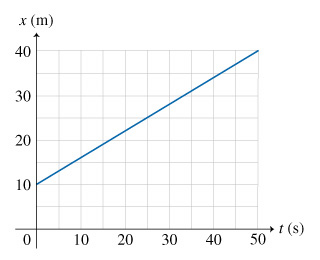
\includegraphics[width=0.5\textwidth]{/Users/max/course-manager/data/semester/Spring 2025/course/PHY2111/chapter/Vectors and Coordinate Systems/section/3.1-3.4/figures/figure_3.jpg}
\end{center}

\setcounter{partcounter}{2}
\paragraph{Parts A-B}

What are the $x$ and $y$ components of the velocity vector?

\begin{solution}
	First, we can make it relative to the axis by
	\[
		\vec{v}_{rel} = \SI{90}{\degree} - \SI{30}{\degree} = \SI{60}{\degree}
		.\]
	Then, we can figure out the angle from the $x$ axis by
	\[
		\SI{180}{\degree} + \SI{60}{\degree} = \SI{240}{\degree}
		.\]
	Compute the $x$ component by
	\[
		v_{x} = 100 \cos 240 = \si{-50}{\degree}
		.\]
	Compute the $y$ component by
	\[
		v_{y} = 100 \sin 240 = \si{-86.6}{\degree}
		.\]
\end{solution}

\newpage

\subsubsection{(Problem 10) Problem 3.27}

\setcounter{partcounter}{1}
\paragraph{Part A}

Find a vector that points in the same direction of the vector $\left( \hat{i} + \hat{j} \right)$ and whose magnitude is $1$.

\begin{solution}
	The magnitude of $\hat{i}$ is 1, and similar with $\hat{j}$.

	We can simply find the normalized vector $v_{n}$ by taking the sum of the magnitudes of the unit vectors $\hat{i}$ and $\hat{j}$ (which are both 1) and dividing each by the root of the sum $M$:
	\begin{align*}
		M &= \sqrt{1 + 1} \\
		v_{n} &= \frac{\hat{i}}{M} + \frac{\hat{j}}{M} \\
		&= \frac{\hat{i}}{\sqrt{2}} + \frac{\hat{j}}{\sqrt{2}}
		.\end{align*}
\end{solution}

\newpage

\subsubsection{(Problem 11) Problem 3.34}

You are fixing the roof of your house when a hammer breaks loose and slides down. The roof makes an angle of \SI{25}{\degree} with the horizontal, and the hammer is moving at \SI{7.5}{m/s} when it reaches the edge. Assume that the hammer is moving from the top of the roof to its right edge.

\setcounter{partcounter}{2}
\paragraph{Parts A-B}

What are the horizontal and vertical components of the hammer's velocity just as it leaves the roof?

\begin{solution}
	Given the angle and the magnitude of the hammer's velocity, this is a simple problem.

	First, the hammer is sliding downwards, so
	\[
		\theta = \SI{360}{\degree} - \SI{26}{\degree} = \SI{335}{\degree}
		.\]

	Since $\cos \theta = \frac{\text{adj}}{\text{hyp}}$ where the hypotenuse is the magnitude of the velocity and the adjacent side is the desired  horizontal component, we can simply solve for the adjacent:
	\begin{align*}
		\cos \SI{335}{\degree} &= \frac{v_x}{\SI{7.5}{\frac{m}{s}}} \\
		v_x &= \SI{7.5}{\frac{m}{s}} \cos \SI{335}{\degree} \\
		&= \SI{6.8}{\frac{m}{s}}
		.\end{align*}
	Similarly,
	\begin{align*}
		v_y &= \SI{7.5}{\frac{m}{s}} \sin \SI{335}{\degree} \\
		&= \SI{-3.2}{\frac{m}{s}}
		.\end{align*}
\end{solution}

\newpage

\subsubsection{(Problem 12) Problem 3.40}

Tom is climbing a \SI{3.0}{m} long ladder that leans against a vertical wall, contacting the wall \SI{2.1}{m} above the ground. His weight of  \SI{680}{N} is a vector pointing vertically downward. (Weight is measured in newtons, abbreviated \SI{}{N}.)

\problempart

What is the magnitude of the component of Tom's weight parallel to the ladder?

~

\begin{solution}

	We can draw a picture of the triangle formed by the ladder and the wall:

	\begin{center}
		\begin{tikzpicture}[>=stealth]

			\tikzmath{
				\scale = 2;
				\yint = 2.1 * \scale;
				\xint = sqrt((3 * \scale)^2 - \yint^2);
				\slope = \yint / \xint;
			};

			\draw[<->] (-0.5,0) -- (\xint + 0.5,0) node[right] {$x$};
			\draw[<->] (0, -0.5) -- (0, \yint + 0.5) node[above] {$y$};
			\draw[] (\xint, 0) -- (0, \yint) node[midway, above right] {\SI{3}{m}};
			\draw[->, densely dashed] (\xint / 2, {(\xint / 2) * \slope}) -- (\xint / 2, 0.5) node[midway, left] {\SI{680}{N}};

			\draw (0, {\yint / 2}) node[left] {\SI{2.1}{m}};
			\draw ({(\xint / 2) + 0.15}, {(\xint / 2 ) * \slope - 0.4}) node[] {$\theta$};
		\end{tikzpicture}
	\end{center}

	We can find theta by using $\cos \theta = \frac{\text{adj}}{\text{hyp}}$:
	\begin{align*}
		\cos \theta &= \frac{2.1}{3} \\
		\theta &= \arccos \left( \frac{2.1}{3} \right) = \SI{45.5729959992}{\degree}
		.\end{align*}
	Then we can figure out the angle relative to the ladder:
	\begin{align*}
		a &= \SI{-45.5729959992}{\degree}
		.\end{align*}
	Therefore, the magnitude of his weight parallel to the ladder is
	\begin{align*}
		\abs{ \SI{680}{N} \cos \left( \SI{-45.5729959992}{\degree} \right) }  &= \SI{476}{N}
		.\end{align*}
\end{solution}

\problempart

What is the magnitude of the component of Tom's weight perpendicular to the ladder?

\begin{solution}
	Similarly, his perpendicular component is simply the $y$ component relative to the ladder:
	\begin{align*}
		\abs{ \SI{680}{N} \sin \left( \SI{-45.5729959992}{\degree} \right) }  &= \SI{485.61}{N}
		.\end{align*}
\end{solution}

\newpage

\subsubsection{(Problem 13) Problem 3.23}

The position of a particle as a function of time is given by $\vec{r} = \left( 6.6 \hat{i} + 4.0 \hat{j} \right)t^2 \SI{}{m}$, where $t$ is in seconds.

~

\setcounter{partcounter}{6}
\paragraph{Parts A-F}

\begin{solution}
	We can find the magnitude $m$ and scale by the time:
	\begin{align*}
		m &= \sqrt{6.6^2 + 4.0^2} = \SI{7.71751255263}{m} \\
		d(t) &= mt^2
		.\end{align*}
	\begin{enumerate}[label=\Alph*.]
		\item $d(0) = \SI{0}{m}$
		\item $d(2.5) = \SI{48.2344534539}{m}$
		\item $d(5.7) = \SI{48.2344534539}{m}$
	\end{enumerate}
	The particle's speed at $t$ is given by
	\begin{align*}
		s(t) &= \abs{ d'(t) } = \abs{ 2mt }
		.\end{align*}
	\begin{enumerate}[label=\Alph*.]
		\setcounter{enumi}{3}
		\item $s(0) = \SI{0}{\frac{m}{s}}$
		\item $s(2.5) = \SI{38.5875627631}{\frac{m}{s}}$
		\item $s(0) = \SI{87.9796431}{\frac{m}{s}}$
	\end{enumerate}
\end{solution}

\newpage

\subsubsection{(Problem 14) Problem 3.25 -- Enhanced -- with Expanded Hints}

\begin{center}
	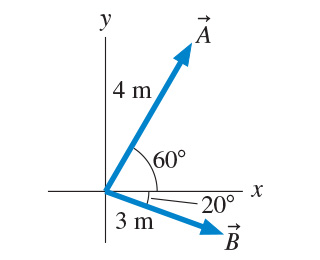
\includegraphics[width=0.5\textwidth]{/Users/max/course-manager/data/semester/Spring 2025/course/PHY2111/chapter/Vectors and Coordinate Systems/section/3.1-3.4/figures/figure_4.jpg}
\end{center}

\setcounter{partcounter}{1}
\paragraph{Part A}

Find vector $\vec{C}$ such that $\vec{A}+\vec{B}+\vec{C}=\vec{0}$. Write your answer in component form.

\begin{solution}
	First, the components of vectors $\vec{A}$ and $\vec{B}$:
	\begin{align*}
		A_{x} &= 4 \cos 60 = 2 \\
		A_{y} &= 4 \cos 60 = 3.46410161514 \\
		B_{x} &= 3 \cos -20 = 2.81907786236 \\
		B_{y} &= 3 \cos -20 = -1.02606042998
		.\end{align*}
	Now, we can solve for $\vec{C}$:
	\begin{align*}
		\vec{C} &= -\vec{A} - \vec{B} \\
		&= -\left( 2, 3.46410161514 \right) - \left( 2.81907786236, -1.02606042998 \right) \\
		&= \left( -4.81907786236, -2.43804118516 \right) \\
		&= -4.81907786236 \hat{i} - 2.43804118516 \hat{j}
		.\end{align*}
\end{solution}

\newpage

\subsubsection{(Problem 15) Problem 3.45 -- Enhanced -- with Expanded Hints}

Four forces are exerted on the object shown in the figure below. The net force on the object is $\vec{F}_{\mathrm{net}} = \vec{F}_{1} + \vec{F}_{2} + \vec{F}_{3} + \vec{F}_{4} = 4.0 \hat{i} \SI{}{N}$.

\begin{center}
	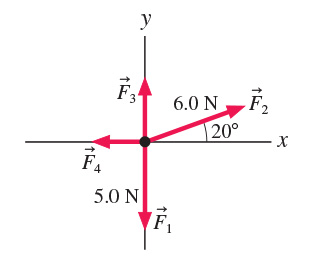
\includegraphics[width=0.5\textwidth]{/Users/max/course-manager/data/semester/Spring 2025/course/PHY2111/chapter/Vectors and Coordinate Systems/section/3.1-3.4/figures/figure_5.jpg}
\end{center}

\setcounter{partcounter}{2}
\paragraph{Parts A-B}

What are the components of  $\vec{F}_{3}$ and $\vec{F}_{4}$?

~

\begin{solution}

	First we will write out the components of the known vectors.
	\begin{align*}
		\vec{F}_{1} &= \left( 0, -5 \right) \\
		\vec{F}_{2} &= \left( 6 \cos 20, 6 \sin 20 \right)
		.\end{align*}
	Since the horizontal component of the net force is zero, we can see that the vertical component of $\vec{F}_{3}$ must be equal and opposite to the sum of the vertical components of $\vec{F}_{1}$ and $\vec{F}_{2}$.
	\begin{align*}
		0 &= \vec{F}_{3y} + \vec{F}_{1y} + \vec{F}_{2y} \\
		\vec{F}_{3y} &= -\vec{F}_{1y} - \vec{F}_{2y} \\
		&= -\left( -5 \right) - \left( 6 \sin 20 \right) = 2.94787914005
		.\end{align*}
	Therefore, $\vec{F}_{3} = \left( 0, 2.94787914005 \right)$.

	We can do something similar for $\vec{F}_{4}$.
	\begin{align*}
		4 &= \vec{F}_{4x} + \vec{F}_{2x} \\
		\vec{F}_{4x} &= 4 - \vec{F}_{2x} \\
		&= -1.63815572472
		.\end{align*}
	Therefore, $\vec{F}_{4} = \left( -1.63815572472, 0 \right)$.
\end{solution}
